

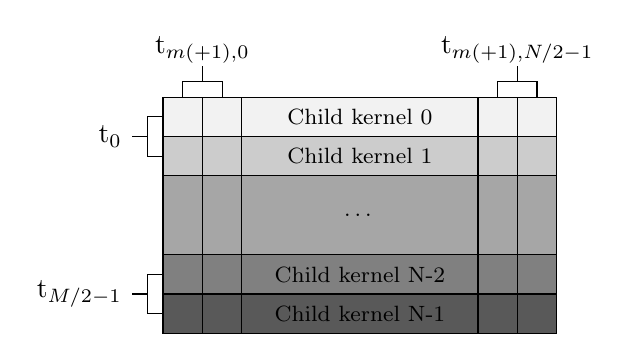
\begin{tikzpicture}[]


%%% GRID %%%%%%%%%%%%%%%%%%%%%%%%%%%%%%%%%%%%%%%%%%%%%%%%%%%%%%%%%%%%%%%%%

\def\rowheight{0.5}
\def\rowwidth{0.5}

\def\delta{0.2};

%%% Grid - lines and fill

\draw[] (0,0) rectangle ++(10*\rowwidth,6*\rowheight);

\filldraw[draw=black, fill=black!05!white] (0,5*\rowheight) rectangle ++(10*\rowwidth,\rowheight);
\filldraw[draw=black, fill=black!20!white] (0,4*\rowheight) rectangle ++(10*\rowwidth,\rowheight);
\filldraw[draw=black, fill=black!35!white] (0,2*\rowheight) rectangle ++(10*\rowwidth,2*\rowheight);
\filldraw[draw=black, fill=black!50!white] (0,\rowheight) rectangle ++(10*\rowwidth,\rowheight);
\filldraw[draw=black, fill=black!65!white] (0,0) rectangle ++(10*\rowwidth,\rowheight);

\draw[] (0,0) rectangle ++(1*\rowwidth,6*\rowheight);
\draw[] (1*\rowwidth,0) rectangle ++(1*\rowwidth,6*\rowheight);
\draw[] (8*\rowwidth,0) rectangle ++(1*\rowwidth,6*\rowheight);
\draw[] (9*\rowwidth,0) rectangle ++(1*\rowwidth,6*\rowheight);


%%% Grid - annotations

\node[black, anchor=center, align=center, font=\footnotesize] at (5*\rowwidth,5.5*\rowheight) {Child kernel 0};
\node[black, anchor=center, align=center, font=\footnotesize] at (5*\rowwidth,4.5*\rowheight) {Child kernel 1};

\node[black, anchor=center, align=center, font=\footnotesize] at (5*\rowwidth,1.5*\rowheight) {Child kernel N-2};
\node[black, anchor=center, align=center, font=\footnotesize] at (5*\rowwidth,0.5*\rowheight) {Child kernel N-1};


%%% Thread annotations

\foreach \i in {0, 4} {

    % Parent
    \draw[black] 
    (0,\i*\rowheight+0.5*\rowheight) --++
    (-\delta,0) --++
    (0,\rowheight) --++
    (\delta, 0);
    \draw[black] (-\delta, \i*\rowheight+1*\rowheight) --++(-\delta, 0);

    % Child
    \draw[black] 
    (\i*2*\rowheight+0.5*\rowheight, 6*\rowheight) --++
    (0, \delta) --++
    (\rowheight, 0) --++
    (0, -\delta);
    \draw[black] (\i*2*\rowheight+1*\rowheight, 6*\rowheight+\delta) --++(0, \delta);

}

\node[black, anchor=east, align=right] at (-2*\delta, 5*\rowheight) {t$_\text{0}$};
\node[black, anchor=east, align=right] at (-2*\delta, 1*\rowheight) {t$_\text{M/2 - 1}$};

\node[black, anchor=south, align=center] at (1*\rowwidth, 6*\rowheight + 1.5*\delta) {t$_\text{m(+1), 0}$};
\node[black, anchor=south, align=center] at (9*\rowwidth, 6*\rowheight + 1.5*\delta) {t$_\text{m(+1), N/2 - 1}$};

\node[black, anchor=center, align=center, font=\footnotesize] at (5*\rowwidth,3*\rowheight) {\dots};


\end{tikzpicture}
